\documentclass[12pt]{article}

\usepackage[a4paper, margin=1in]{geometry} % Margins
\usepackage{fancyhdr} % Set header and footer
\usepackage{titling}

\usepackage[T1]{fontenc} % For international characters
\usepackage{XCharter} % XCharter as the main font

\usepackage[
  backend=biber,
  style=numeric,
  citestyle=authoryear,
  sorting=none
  ]{biblatex}
\addbibresource{./Ref/reference.bib}

\usepackage[english]{babel} % Use english by default
\usepackage{csquotes}

\usepackage{amsmath, amsthm, amssymb, amsfonts, mathtools}
\usepackage{graphicx}
\usepackage{tikz}
\usetikzlibrary{shapes, arrows}
% \usepackage[]{algorithm2e}
% \usepackage{caption, enumerate}
% \usetikzlibrary{graphdrawing, shapes}
% \usegdlibrary{trees}

\usepackage{hyperref}
\hypersetup{
  colorlinks,
  citecolor=black,
  filecolor=black,
  linkcolor=black,
  urlcolor=black
}

\pagestyle{fancy}
\fancyhf{}
\fancyhead[R]{Leo W.}
\fancyfoot[R]{\thepage}
\setlength{\headheight}{15pt}

%----------------------------------------------------------------------------------------
%	CUSTOM COMMANDS
%----------------------------------------------------------------------------------------

\newcommand{\articletitle}[1]{\renewcommand{\articletitle}{#1}} % Define a command for storing the article title
\newcommand{\articlecitation}[1]{\renewcommand{\articlecitation}{#1}} % Define a command for storing the article citation
\newcommand{\doctitle}{\articlecitation\ --- ``\articletitle''} % Define a command to store the article information as it will appear in the title and header
\newcommand{\doctitlenocite}{\articletitle} % No citation

\newcommand{\datenotesstarted}[1]{\renewcommand{\datenotesstarted}{#1}} % Define a command to store the date when notes were first made
\newcommand{\docdate}[1]{\renewcommand{\docdate}{#1}} % Define a command to store the date line in the title

\newcommand{\docauthor}[1]{\renewcommand{\docauthor}{#1}} % Define a command for storing the article notes author

\newcommand{\bookcitation}[1]{\renewcommand{\bookcitation}{#1}} % Define a command for storing the book citation

% Define a command for the structure of the document title
\newcommand{\printtitle}{
\begin{center}
\textbf{\Large{\doctitle}}

\docdate

\docauthor
\end{center}
}

% No citation
\newcommand{\printtitlenocite}{
\begin{center}
\textbf{\Large{\doctitlenocite}}

\docauthor

\docdate
\end{center}
}

%----------------------------------------------------------------------------------------
%	STRUCTURE MODIFICATIONS
%----------------------------------------------------------------------------------------

\setlength{\parskip}{3pt} % Slightly increase spacing between paragraphs

% Uncomment to center section titles
% \usepackage{sectsty}
% \sectionfont{\centering}

% Uncomment for Roman numerals for section numbers
% \renewcommand\thesection{\Roman{section}}
% \renewcommand\thesubsection{\thesection.\Roman{subsection}}


\title{Introductory Backtesting Notes \\ for Quantitative Trading Strategies \\[2ex]
  \large Maybe Some Eye-catching Subtitle}
\author{Leo Wong (QFIN \& COSC, HKUST)}
\date{September, 2019}

\begin{document}

\begin{titlingpage}
  \maketitle
  \begin{abstract}
    \enquote{All models are wrong, but some are useful}, \cite{allmodelsarewrong}. This note is compiled for COMP4971C in Fall 2019 to assist the research of quantitative trading strategies.
  \end{abstract}
\end{titlingpage}

\fancyhead[L]{Introductory Backtesting Notes}

\tableofcontents

\section{Introduction}

Backtesting is a compulsory stage in the development of any quantitative trading strategies. It evaluates the performance of a strategy with historical data and provides the following usages:

\begin{enumerate}
  \item validate the effectiveness of the trading idea
  \item tune the parameters of the strategy
  \item predict the future performance (assuming repeating market patterns)
\end{enumerate}

This note briefly introduces some industrial practices in backtesting a quantitative trading strategy for general first order securities (e.g. equity share, commodity future, etc.) along with some common mistakes. The majority of the content comes from several books and articles including but not limited to \cite{insideblackbox}, \cite{succalgotrading}, \cite{epchan2008}. All references are listed at the end of the note.

The structure diagram of a suggested backtest system is included below.

\tikzset{%
  block/.style    = {draw, thick, rectangle, minimum height = 3em, minimum width = 3em},
  sum/.style      = {draw, circle, node distance = 2cm}, % Adder
  input/.style    = {coordinate}, % Input
  output/.style   = {coordinate} % Output
}
% Defining string as labels of certain blocks.
\newcommand{\suma}{\Large$+$}
\newcommand{\inte}{$\displaystyle \int$}
\newcommand{\derv}{\huge$\frac{d}{dt}$}

\begin{tikzpicture}[auto, thick, node distance=2cm, >=triangle 45]
  \node at (2, 11) {\textsc{\large Structure of Backtest System}};
  \draw [thick] (1, 0) rectangle (13, 10);

  \draw node at (-1, 5) [block, name=data] {Data};
  \draw node at (3, 8) [block, name=alpha] {Alpha Model};
  \draw node at (6, 8) [block, name=risk] {Risk Model};
  \draw node at (10, 8) [block, name=cost] {Transaction Cost Model};
  \draw node at (7, 5) [block, name=portfolio] {Portfolio Construction Engine};
  \draw node at (7, 2) [block, name=execution] {Execution Engine};

  \draw[->] (data) -- (1, 5);
  \draw[->] (alpha) -- (portfolio);
  \draw[->] (risk) -- (portfolio);
  \draw[->] (cost) -- (portfolio);
  \draw[<->] (portfolio) -- (execution);

\end{tikzpicture}

\section{Note and Assumption}

\begin{enumerate}
  \item All \enquote{suggested} values are annualized, calculations are stated below
  \item All \enquote{suggested} values are calculated after deducting transaction cost
  \item Returns at different time \(t\) are assumed to be IID \footnote{Independent and identically distributed, i.e. assuming same probability distribution and mutually independent}, otherwise the estimation of Sharpe ratio from sample needs to be adjusted accordingly
\end{enumerate}

\section{Primary Metrics}

Primary metrics should be used for all types of trading strategies.

\subsection{Sharpe Ratio}

\subsubsection*{Metric Introduction}

Sharpe ratio is first introduced by \cite{sharpe1966}. Its original name \enquote{Reward-to-Variability Ratio} reflects its nature of balancing return and risk of a strategy. According to the definition in \cite{sharpe1994}, assume \(R_{Pt}\) as a \(t\)-period return series, \(R_{ft}\) as the risk-free rate series over the same period. Then the Sharpe ratio \(S_h\) from \(t=1\) to \(t=T\):

\begin{align*}
  S_h &\equiv \frac{\overline{D}}{\sigma_D} \\
  \text{where}~D &\equiv R_{Pt} - R_{ft} \\
  \overline{D} &\equiv \frac{1}{T} \sum_{t=1}^T D_t \\
  \sigma_D &\equiv \sqrt{\frac{\sum_{t=1}^T (D_t-\overline{D})^2}{T-1}}
\end{align*}

This Sharpe ratio indicates the historical average differential return per unit pf historical variability of the differential return (\cite{sharpe1966}). In simpler terms, Sharpe ratio measures the expected return gained per unit of risk taken for a zero investment strategy. The Sharpe ratio does not cover cases in which only one investment return is involved (\cite{sharpe1994}).

\subsubsection*{Suggested Level}

\begin{figure}[h!]
  \centering
  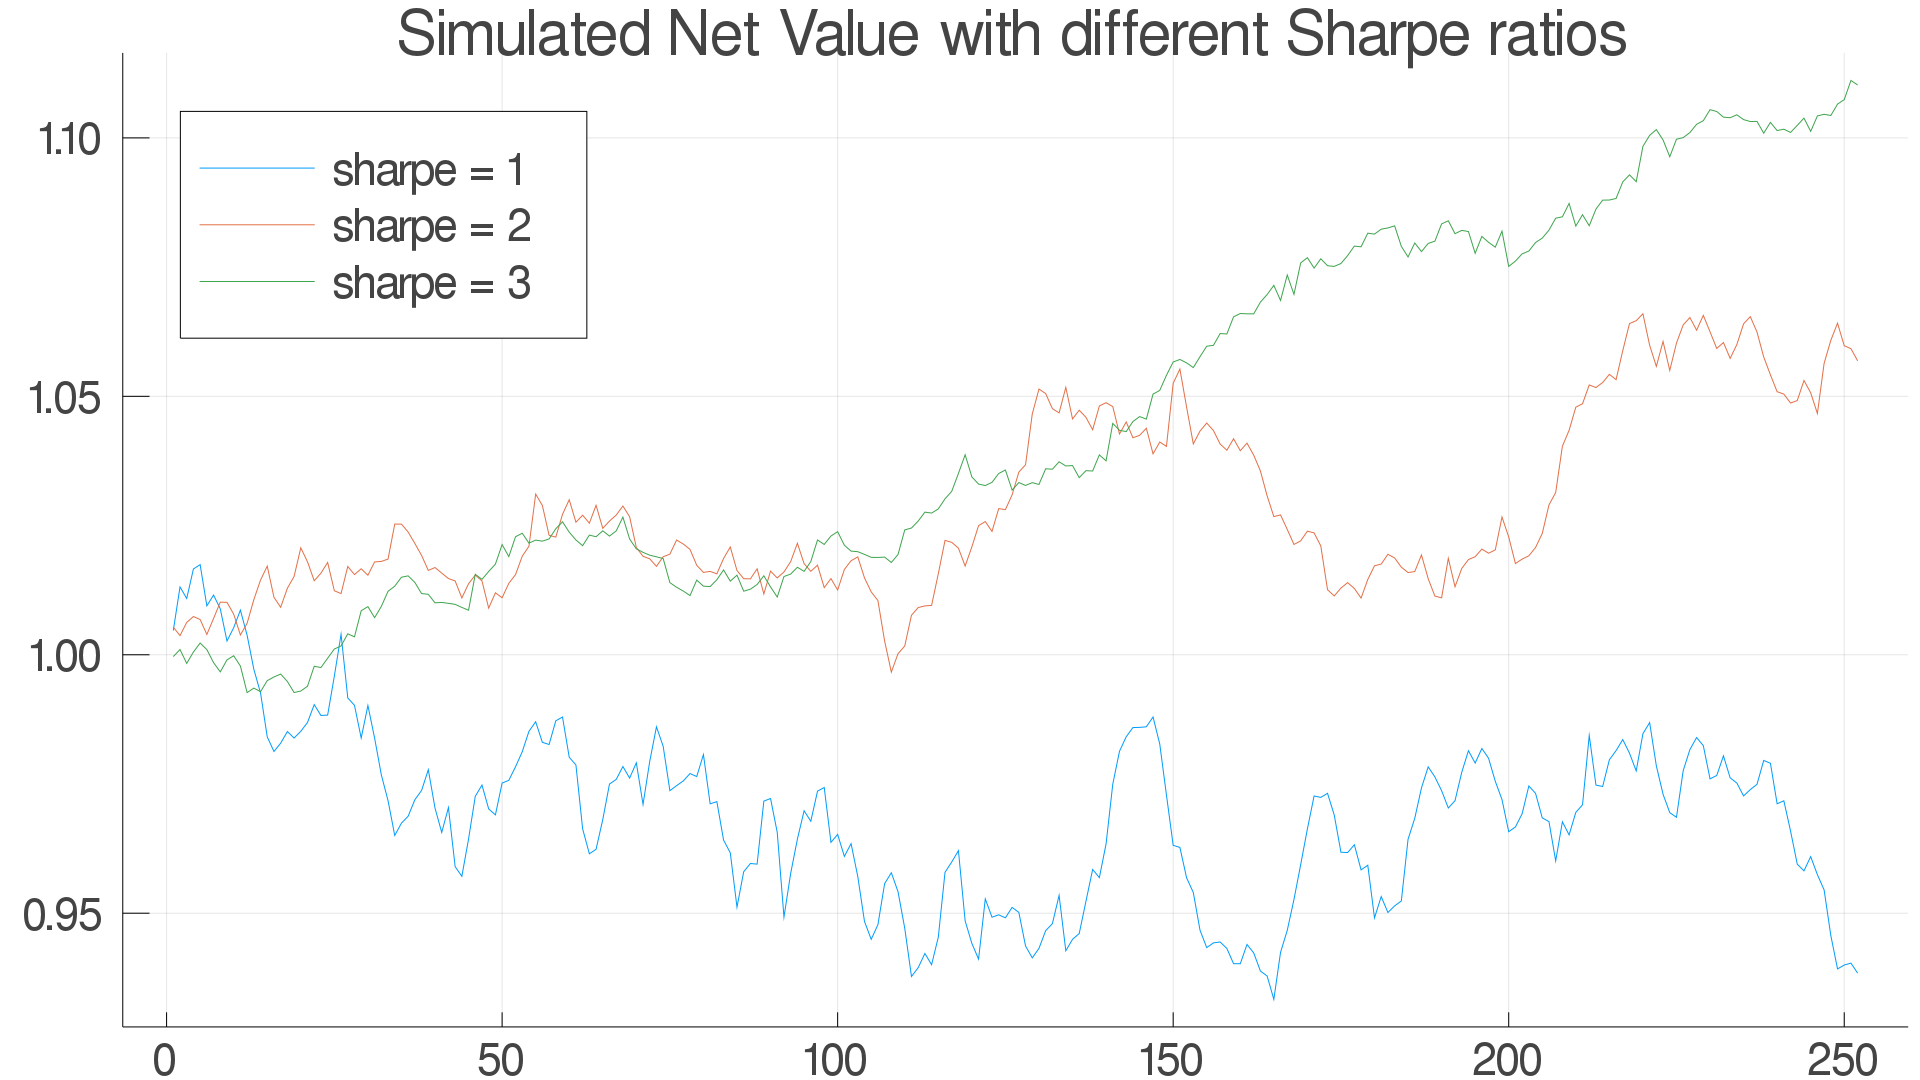
\includegraphics[scale=0.22]{./ref/figure/sharpe_nav_1080.png}
  \caption{Net value graph of multiple sharpe ratios}
  \label{fig:sharpe_navs}
\end{figure}

The above diagram shows 3 different return series of Sharpe ratios ranging from 1 to 3, with 252 steps (simulating year-long daily returns). For a day-frequency strategy, \(S_h > 1\) usually is not enough to generate consistent profits. A Sharpe value greater than 1.5 or even 2 is recommended. For longer-frequency strategies (i.e. weekly, monthly), \(S_h > 0.7\) can be acceptable, \(S_h > 1.2\) can be regarded as very good.

All values in the above section should be treated as reference instead of absolute limit/standard to judge a strategy.

\subsection{Maximum Drawdown}

\subsubsection*{Metric Introduction}

Maximum drawdown is a specific measure of drawdown (the peak-to-trough decline during a specified timespan) that measures the greatest decline from a peak, before a new peak is reached.

\begin{align*}
  MDD &= \min DD_i \tag*{where \(i \in {\{0, ..., T \}} \)} \\
  DD_t &= \frac{V_t}{\max \{V_0, V_1, ..., V_t \}}-1 \tag*{for \(t \in {\{0, ..., T \}} \)}
\end{align*}

Note that it only measures the size of the largest loss, not the frequency of large losses. MDD does not indicate how long it took an investor to recover from the loss, or if the investment even recovered at all.

\subsubsection*{Suggested Level}

insert (maximum) drawdown figure

\subsection{Profit Factor, Win Rate and Payoff Ratio}

\subsubsection*{Metric Introduction}

Let \(\pi_t\) be the profit/loss of a strategy at time \(t\), \(T\) be the total number of steps (timespan). Assume the profit/loss is non-zero at every time \(t\), i.e. \(n_{\pi=0} = 0\), then \(T = n_{\pi<0} + n_{\pi>0}\). Let \(w\) be the win rate, \(pf\) be the profit factor, \(pr\) be the payoff ratio, \(RoR\) be the risk of ruin.

\begin{align*}
  w &= \frac{pf}{pf+pr} \\
  \text{where}~w &\equiv \frac{n_{\pi>0}}{n_{\pi<0} + n_{\pi>0}} \\
  pf &\equiv \frac{\sum_{t, \pi_t>0} \pi_t}{\sum_{t, \pi_t<0} \pi_t} \\
  pr &\equiv \frac{\sum_{t, \pi_t>0} \pi_t}{\sum_{t, \pi_t<0} \pi_t} \cdot \frac{n_{\pi<0}}{n_{\pi>0}}
\end{align*}

lorem

\begin{align*}
  RoR &= (1-w)^R
\end{align*}

lorem

\subsubsection*{Suggested Level}

lorem

\section{Secondary Metrics}

Secondary metrics provide easy explanation for non-finance-heavy personnel.

\subsection{Compound Annual Growth Rate (CAGR)}

\subsubsection*{Metric Introduction}

Compound annual growth rate (CAGR) is the annualized, required rate of return for an investment to grow in timespan \(T\) (in years), assuming the intermediate profits are reinvested.

\begin{align*}
  CAGR = \bigg(\frac{V_T}{V_0} \bigg)^{\frac{1}{T}}-1
\end{align*}

CAGR is not the true rate of return, but rather a smoothed, representational figure, usually used for easier explanation and comparison.

\subsubsection*{Suggested Level}

The desired CAGR depends on the nature of the security and even its sector. Different types of securities (e.g. equity, fixed income, index, derivative) have different return characteristics.

\subsection{Volatility of Return}

\subsubsection*{Metric Introduction}

lorem

\begin{align*}
  y = f(x)
\end{align*}

lorem

\subsubsection*{Suggested Level}

lorem

\subsection{Maximum Drawdown Duration}

\subsubsection*{Metric Introduction}

lorem

\begin{align*}
  y = f(x)
\end{align*}

lorem

\subsubsection*{Suggested Level}

lorem

\section{Common Pitfall}

This section introduces multiple common mistakes made by quants in backtest.

\subsection{Survivorship Bias}

lorem

\subsection{Transaction Costs}

lorem

\subsection{Market Nature/Pattern}

lorem

\subsection{Look Ahead Bias}

lorem

\subsection{Overfitting}

lorem

\section*{Conclusion}

lorem

\renewcommand{\refname}{Reference} % Change the default bibliography title
\printbibliography

\end{document}
